%%%%%%%%%%%%%%%%%%%%%%%%%%%%%%%%%%%%%%%%%%%%%%%%%%%%%%%%%%%%%%%%%%%%%%%%
% Plantilla TFG/TFM
% Escuela Politécnica Superior de la Universidad de Alicante
% Realizado por: Jose Manuel Requena Plens
% Contacto: info@jmrplens.com / Telegram:@jmrplens
%%%%%%%%%%%%%%%%%%%%%%%%%%%%%%%%%%%%%%%%%%%%%%%%%%%%%%%%%%%%%%%%%%%%%%%%

\chapter{Fluid Mechanics: specificities}
\label{fluid_mechanics}

\section{Low Reynolds flow}

The Reynolds number is a dimensionless number widely used in fluid mechanics.

Although George Gabriel Stokes already introduced this number in 1851, it was named after the irish physicist, Osborne Reynolds, who popularized its use 3 years later.

Several interpretations of this number can be given (see, for instance, Lauga and Power~\cite{Lauga}). The most classic amongst them is at its origin: the quantification of the relative importance of the viscous and inertial terms in the Navier-Stokes equations.

Without external forces, the momentum equation reads as follows:

\begin{equation}
\begin{aligned}
& \rho \frac{\partial \mathbf{v}}{\partial t} \quad + \\
\sim & \rho_c \frac{u_{ci}}{t_c} 
\end{aligned}
\begin{aligned}
& \rho v (\nabla v) \quad = \\
\sim & \rho_c \frac{u_{ci}^2}{l_{ci}}
\end{aligned}
\begin{aligned}
& \nabla p \quad + \\
\sim & \frac{\Delta_i p}{l_{ci}}
\end{aligned}
\begin{aligned}
& \nabla \cdot \overline{\overline\tau}' \\
\sim & \mu_c \frac{u_{ci}}{l_{cmin}^2}
\end{aligned}
\label{CDM}
\end{equation}

Under Eq. \ref{CDM} the orders of the different terms have been specified. One can now compare the aforementioned terms, which leads to the expression of the Reynolds number:
\begin{equation}
	Re = \rho_c u_c l_c/\mu_c
\end{equation}

Thus, when the Reynolds number is very low, one can neglect the inertial terms, and vice versa. This hierarchization of terms allows drastically simplifying the NS equations, which is very useful given that the Navier–Stokes existence and smoothness problem remains unsolved.

Stokes equations (see Eq. \ref{stokes_f}) constitute the zero Reynolds limit to the NS equations, provided that there is no forcing term or that the forcing term is also negligible ($Sr<<1$). These equations, as opposed to NS, are linear. For a certain geometry and boundary conditions, this grants a certain number of properties to the flow that can be described by them:

\begin{itemize}
	\item Uniqueness of the solution  
	\item Minimum dissipation
	\item Additivity and reversibility
\end{itemize}

The last of these properties allows us to describe the flow by means of the superposition of different fundamental solutions such as the Stokeslet or the Stresslet, as explained on previous sections.

\section{2-Dimensional flow}

When trying to find out the velocity field around a sphere of radius $a$ under uniform flow, $U_\infty$, in the low Reynolds world, we obtain the following axisymmetric solution in spheric coordinates:

\begin{equation}
\psi = U_\infty \left(\frac{r^2}{2} - \frac{3}{4}ar + \frac{1}{4} \frac{a^3}{r} \right) sin ^2 \theta
\left\{
\begin{aligned}
& u_r = \frac{1}{r^2 sin \theta} \frac{\partial \psi}{\partial \theta}\\
& u_\theta = \frac{-1}{r sin \theta} \frac{\partial \psi}{\partial r}
\end{aligned}
\right.
\end{equation}

where $\psi$ is the stream function.

However, if we study this solution, we come across a contradiction if we compare the advective and viscous terms:


It turns out that in the far field, the inertial terms cannot be neglected anymore.

What is more, if we now try to find the flow field around an infinite cylinder (or around a circle in 2D), a valid solution does not even exist in the flow field. This is known as the Stokes paradox.

Later, a correct solution for a cylinder was derived using Oseen's equations. 

It should be however noted that, as a consequence of this paradox, perturbations (i.e.:presence of obstacles,...) are longer ranged in 2D than in 3D. Hence our present study. 

\section{Films}

In their article, Sonin et al.~\cite{SONIN1994} consider a 1mm diameter film, consisting of a flat part which is liked to the surrounding wire by a meniscus-shaped contour. The diameter of this flat part is fixed by the value of a pressure $P_i$ that corresponds the air pressure in a reservoir linked to the film. Since we want our measurements to be taken in 2D films, in this section we will try to understand what determines the extent of the flat part, if it exists, in the absence of such a reservoir.

\subsection{Definitions}

In order to make the following section a bit more understandable for engineers or scientists with little or no background in this field, we will start by explaining some fundamental concepts.

\subsubsection{Surface tension}

The \textbf{surface tension} or \textbf{surface energy} is, from a thermodynamic point of view, the energy needed to increase a liquid's interface by unit area. Fluid mechanics provides us with another description: as a force per unit length, tangent to the surface, that keeps it together.

At air-liquid interfaces, the origin of surface tension is usually explained with the help of the following diagram:

\begin{figure}[H]
	\centering
	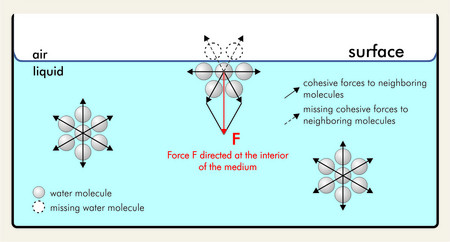
\includegraphics[width=0.6\textwidth]{archivos/surface_tension.png}
	\caption[Caption for LOF]{Illustration of the cohesive forces that result in the surface tension\protect\footnotemark~\cite{sita-process}}
	\label{surface_tension}
\end{figure}

\footnotetext{As it is explained later in this section, this figure is incomplete.}

Within the liquid bulk, a molecule is subject to cohesion forces upon its neighboring particles. They completely surround it resulting in a force equilibrium on that molecule.

Nevertheless, when a molecule belongs to a surface, this symmetry is broken and so does the equilibrium, leading to an increase of the free energy.

But then, 

\begin{displayquote}
	\textit{Why is surface tension a force parallel to the interface while it is so obvious that it must be perpendicular to it?}
\end{displayquote}

This question can be found in ??? Snoeijer 2011 ???. Also provided in the aforementioned article is this short answer:

\begin{displayquote}
	\textit{The schematic of Fig. \ref{surface_tension} represents only the attractive intermolecular forces. The real force balance requires both repulsive and attractive interactions between liquid molecules.}
\end{displayquote}

as well as an exhaustive explanation that we will not detail in this document.  

On a more practical level, E\"{o}tv\"{o}s rule allows us to calculate the approximate value of a liquid's surface tension, $\gamma$, as:

\begin{equation} 
\gamma V_m^{2/3}=k\left(T_{c}-T-6\right)
\label{eotvos}
\end{equation}

where $V_m$ is the molar volume, $T_c$ is the critical temperature of the liquid, and $k$ is the Eötvös constant. It has a value of $2.1\cdot 10^{-7} \; \frac{\textrm{J}}{\textrm{K} \cdot \textrm{mol}^{\textrm{2/3}}}$ no matter the liquid.

The resulting value for water at $25^\textrm{o} \textrm{C}$ is $7.17 \cdot 10^{-2} \; \textrm{N/m}$.

\subsubsection{Capillary pressure}

The \textbf{capillary pressure} between two immiscible fluids is defined as:

\begin{equation} 
	p_c = p_{nw} - p_{w}
	\label{cap_pressure}
\end{equation}

where $nw$ and $w$ stand respectively for the non-wetting and wetting phases, meaning $P_c$ represents a pressure jump across the interface. Throughout this section our wetting liquid will be water and the air will be the non-wetting phase. This combination has been extensively studied due to its countless applications.

We will consider that the ambient pressure is known, so we can use equation \ref{cap_pressure} to calculate the pressure on liquid side of the interface. However, we first need the value of the capillary pressure, which is given by the Young-Laplace equation:

\begin{equation} 
p_c = -\gamma \nabla \cdot \hat{n} = 2 \gamma H
\label{young_laplace}
\end{equation}

$H$ being the mean curvature (average of the principal curvatures):

\begin{equation} 
2H = \frac{1}{R_1} + \frac{1}{R_2}
\label{curvature}
\end{equation}

\subsection{Shape of the interface: energetic considerations}

Looking through the literature we found some descriptions of the real shape of the liquid-air interface in contact with a solid wall. 

Generally, two different cases are considered: either the gravity plays an important role or it does not.

An analytic description of the shape resulting of the balance between gravitation and the Young-Laplace pressure drop at the curved surface can be found in the book \textit{Statistical Thermodynamics of Surfaces, Interfaces, and Membranes} by Safran~\cite{Safran}.

When it comes to assessing the case where gravitational forces are negligible, and given there are no other forces, the Young-Laplace pressure drop has to be constant in all the surface. This is because, in a static equilibrium situation, the pressure within the bulk of the liquid has to be uniform. Moreover, if boundary conditions are symmetric with respect to an axis, the shape of the meniscus will hold the same symmetry. 

In his paper, Princen~\cite{PRINCEN1970} calculates the shape and size of the cross section of \textit{Liquid Columns between Horizontal Parallel Cylinders}. For the pressure drop to be uniform, and since one of the radius of curvature is infinite, the other one has to be constant. Therefore, the shape of the free surface is a right circular cylinder.

\begin{figure}[H]
	\centering
	\includegraphics[width=0.3\textwidth]{archivos/drop_column.png}
	\caption{Cross section of a liquid column between two horizontal rods} 
	\label{drop_column}
\end{figure}

To find the value of $R$, the energetic balance proposed by Princen (see Eqs. \ref{princen_eq}) confronts the \textit{free energy $dF$ associated with injecting an infinitesimal volume dV (e.g., from a hypodermic syringe) into the liquid column} with the \textit{work $dW$ done on the system (including the syringe) as a result of the pressure difference across the piston}.

\begin{equation}
\begin{aligned} &\mathrm{d} F=[(AB+CD)-(AC+BD) \cos \theta_0 ] \gamma \mathrm{d} L \\
& \mathrm{d} W= p_c \mathrm{d} V=-\gamma A_{cs} \mathrm{d} L / R \end{aligned}
\label{princen_eq}
\end{equation}

where $A_{cs}$ is the cross-sectional area of the water column.

For such a case, the further addition of liquid does not change the cross section, but only the length of the column. Our geometry, on the contrary, sees its cross area unavoidably dilated because its length is fixed.

This is why we still want to consider another approach: we consider a layer, whose surface is described by the Monge representation. The free energy of the water-air interface is:

\begin{equation}
F_{s}=\int \int d x d y\left[\gamma \sqrt{1+h_{x}^{2}+h_{y}^{2}}\right]
\end{equation}
 
We ignore the energy of the surface between the solid and the wetting phase, assuming that it is negligible since its surface is much smaller. 

To be able to solve it analytically, we are going to consider a circular film instead of a square shaped one. In that case, the orders of magnitude of the aforementioned energies are: 

\begin{equation}
\left\{
\begin{aligned} & F_{air-liquid} = \gamma s_{air-liquid} \sim \gamma \times 2 \times \pi R^2 \sim 4 \cdot 10^{-6} \; \textrm{J} \\
& F_{solid-liquid} = \gamma s_{solid-liquid} \cos \theta  < \gamma \times 2 \pi R \times \pi \rho \sim 1 \cdot 10^{-7} \; \textrm{J}
\end{aligned}
\right.
\end{equation}

where $s_{air-liquid}$ and $s_{solid-liquid}$ are the areas of both interfaces, $R = 3 \; \textrm{mm}$ is the radius of the film, $\rho = 25 \; \mu \textrm{m}$ is the radius of the surrounding thread, and $\theta = 70^\textrm{o}$ is the contact angle between water and nylon. In conclusion, neglecting $F_{solid-liquid}$ seems to be a rather good approximation.

We are now going to minimize the free energy under the constraint of fixed volume using the Euler-Lagrange equation (see Eq. \ref{EulerLagrange}) with a Lagrange multiplier, $\lambda$. The function to minimize is:

\begin{equation}
G=2 \pi \gamma \int_{0}^{R} r\left(1+h_r^{2}\right)^{1 / 2} d r-\lambda 2 \pi \int_{0}^{R} r h d r
\end{equation}

And the Euler-Lagrange equation reads:

\begin{equation}
\frac{\partial f}{\partial h} - \frac{d}{d r}\left(\frac{\partial f}{\partial h_r}\right) = 0
\end{equation}

where, in this case:

\begin{equation}
f\left(h, h_r, r\right)=\gamma r\left(1+h_r^2\right)^{1 / 2}-\lambda r h
\label{EulerLagrange}
\end{equation}

We can now calculate both terms:

\begin{equation}
\left\{\begin{array}{l}{\frac{\partial f}{\partial h}=\lambda r} \\ {\frac{\partial f}{\partial h_r}=\gamma r \frac{h_r}{\left(1+h_r^2\right)^{1/2}} \rightarrow \frac{d}{d r}\left(\frac{\partial f}{\partial h_r}\right)=\gamma\left[\frac{h_r}{\left(1+h_r^{2}\right)^{1/2}}+\frac{r h_{rr}}{\left(1+h^{2}\right)^{1 / 2}}-\frac{r h_r^{2} h_{rr}}{\left(1+h_r^{2}\right)^{3 / 2}}\right]}\end{array}\right.
\label{TermsEL}
\end{equation}

However, before inserting them in Eq. \ref{EulerLagrange}, we need to recall that our Young-Laplace pressure jump must be constant in the whole surface, which leads to the following constraint:

\begin{equation}
\frac{h_{rr}}{\left(1+h_r^{2}\right)^{3 / 2}}-\frac{\sin \left(\operatorname{atan}\left(h_r\right)\right)}{r}=C
\label{PressureConstraint}
\end{equation}

where $C$ is a constant.

We can now simplify the terms in \ref{TermsEL} with the help of \ref{PressureConstraint} and insert them in Eq. \ref{EulerLagrange}, which leads to:

\begin{equation}
h^{\prime}=\frac{\frac{1}{2}\left(\frac{\lambda}{\gamma}-C\right) r}{\sqrt{1-\frac{1}{4}\left(\frac{\lambda}{\gamma}-C\right)^{2} r^{2}}}
\end{equation}

In this equation we notice, that, as a consequence of axial symmetry and continuity, the derivative goes to zero when $r$ goes to zero. From now on, we will use the letter $B$ to express the constant $\frac{1}{2}\left(\frac{\lambda}{\gamma}-C\right) R$. Integration of the expression above leads to:

\begin{equation}
h^{\prime}=\frac{B \frac{r}{R}}{\sqrt{1-B^{2} \left(\frac{r}{R}\right)^2}} \rightarrow h=-\frac{\sqrt{1-B^{2} \left(\frac{r}{R}\right)^2}}{B} R + K
\end{equation}

where $K$ is a constant.

To find our constants we need to impose the corresponding constraints. The constraint over the volume can be replaced with another determining the value of $h$ in the center of the film, where we want $h$ to be half of the desired thickness:

\begin{equation}
h(r=0) = \frac{t}{2} = h_0 \rightarrow K = \frac{R}{B} + h_0
\end{equation}

\begin{figure}[H]
	\centering
	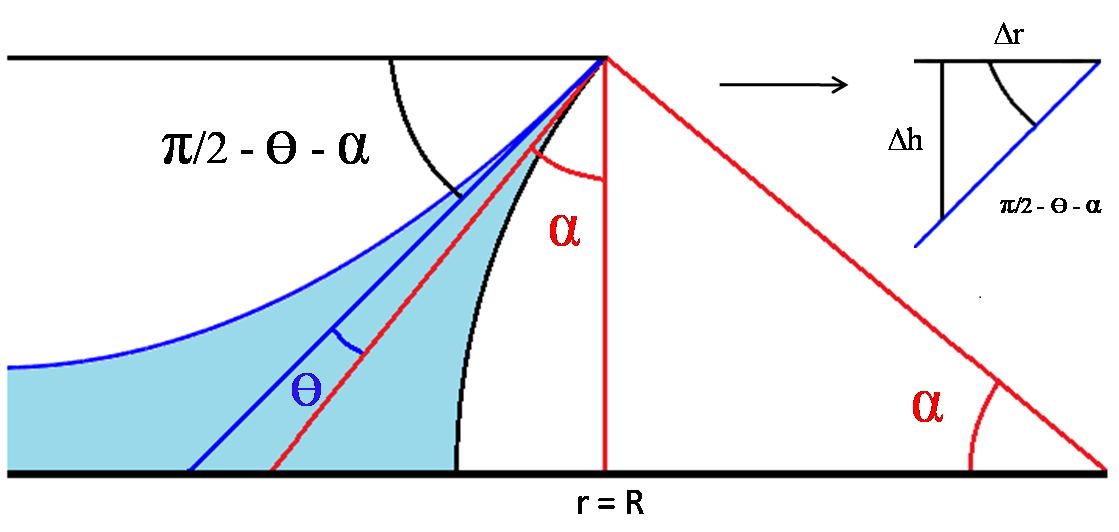
\includegraphics[width=0.7\textwidth]{archivos/geom_film.png}
	\caption{Diagram of a the liquid film next to the thread.}
	\label{geom_film}
\end{figure}

The second constraint is the contact angle between the liquid and the solid. Fig. \ref{geom_film} helps us find out the expression of this constraint:

\begin{equation}
h_r(r=R)=\tan \left(\frac{\pi}{2}-\theta-\alpha\right) 
\end{equation}

where $\alpha=\textrm{asin} \left[\frac{h(r=R)}{\rho}\right]$. This leads to:

\begin{equation}
\tan[(\operatorname{asin}[B])] = \tan \left[[\frac{\pi}{2}-\theta-\operatorname{asin}\left(-\frac{\sqrt{1-B^{2}}}{B} \frac{R}{\rho}+\frac{1}{B}\frac{R}{\rho}+\frac{h_0}{\rho}\right)\right]
\end{equation}

Since $\|B\|$ has to be smaller than one for it to have a solution, this equation can be rewritten as:

\begin{equation}
\sin \left(\frac{\pi}{2} - \theta \right) (1 - B^2)^{1/2} B - \cos \left(\frac{\pi}{2} - \theta\right) B^2 = - [(1 - B^2)^{1/2}+1] \frac{R}{\rho} + \frac{h_0}{\rho} B
\end{equation}

For the values $R = 3 \; \textrm{mm}$, $\rho = 25 \; \mu \textrm{m}$ and $\theta = 70^\textrm{o}$, $h_0 = t/2 = 7.5 \; \mu \textrm{m}$, which are similar to the dimensions of our film, we obtain $B \simeq 6.90 \cdot 10^{-4}$ and a volume of $ \simeq 0.45 \; \mu \textrm{L}$. The shape of the film is shown in the next figures:

\begin{figure}[H]
	\centering
	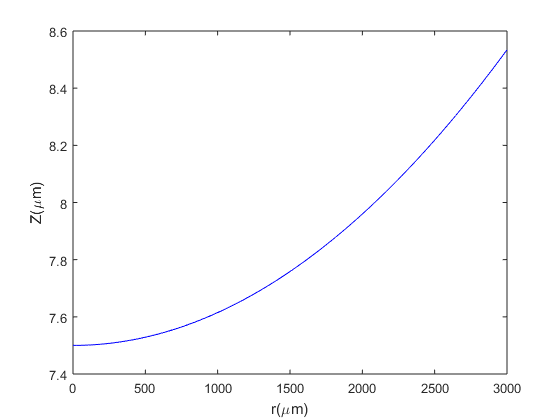
\includegraphics[width=0.6\textwidth]{archivos/CircFilmFunction.png}
	\caption{Half thickness of the film as a function of the radial position.}
	\label{CircFilmFunction}
\end{figure}

\begin{figure}[H]
	\centering
	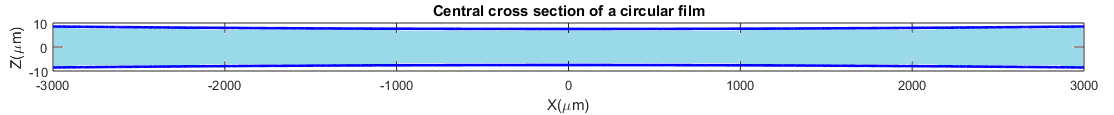
\includegraphics[width=\textwidth]{archivos/CircFilmSection.png}
	\caption{Diagram of a the liquid film next to the thread.}
	\label{CircFilmSection}
\end{figure}

Far enough from the boundary conditions we can expect a similar shape for a square shaped film, so indeed we can consider that it is mostly flat.

\section{Surfactants}

A surfactant is a chemical substance that, when used as a solute, reduces the surface tension of the colloid. Hence, they are also called surface-active agents.
 
Surfactant molecules have at least one portion of their structure that is hydrophobic and one part that is hydrophilic. It is this duality that gives them their unique properties.
 
These substances reduce the surface tension of their solvent by acting like an inter-phasial bridges between the fluid and the air. In fluids like water the hydrophilic portion of the molecule will orient itself towards the fluid, while the hydrophobic portion will point outwards. This accommodation reduces the total amount of energy needed in to form the surface of the fluid, thus reducing the surface tension.
 
Surfactants may also form aggregates, normally spherical, called micelles. In this assemblies of molecules, the hydrophilic parts form the outer layer of the sphere while the hydrophobic groups point inwards avoiding direct contact with the solvent.

\section{Flowing films}

As we will see later, in the ¿¿¿Results and Analysis??? section, flows unrelated to algae motion (what we call \textit{background flows}) have been an important issue in this research.

To understand them, we looked for bibliography on several topics, among which, flowing films (see Fig. \ref{flowing_film}).

We developed some equations for our problem (quasi-horizontal layer) based on Rutgers' 2D model ¿¿¿ Rutgers 1998 ??? of a falling vertical film. This model an air box of width L through and thickness 2d around the film and calculates both the velocity field in the air and the film. Motion is not driven, as usual, by a pressure gradient, but by the force of gravity on the film.

\begin{figure}[H]
	\centering
	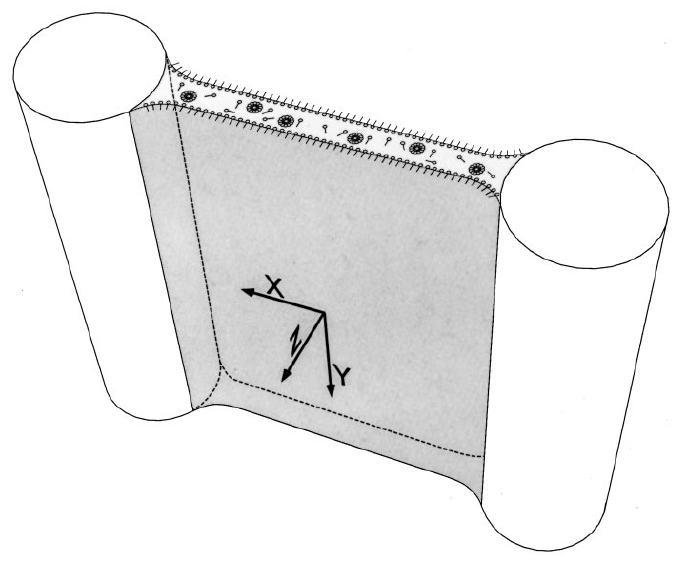
\includegraphics[width=0.4\textwidth]{archivos/FilmBetweenWires.png}
	\caption{Diagram of a liquid film between two wires~\cite{Rutgers2001}. The \textit{head and tail} structures represent molecules of surfactant.}
	\label{flowing_film}
\end{figure}

This model constitutes a very simplified approach, because it is obvious that our boundary conditions are going to have an important effect (i.e. our fluid is never renewed, but it recirculates), but it should at least give us an idea of the magnitudes in our problem.

The equation for the surrounding air reads :

\begin{equation}
\frac{\partial^{2} v_{\mathrm{a}}(x, z)}{\partial x^{2}}+\frac{\partial^{2} v_{\mathrm{a}}(x, z)}{\partial z^{2}}=0
\label{air_velocity}
\end{equation}

And the one for the film itself:

\begin{equation}
\mu_{2D} \frac{d^{2} v(x)}{d x^{2}}=-2 \mu_{\mathrm{a}}\left|\frac{\partial v_{a}(x, z)}{\partial z}\right|_{z=0^{+}}-\rho h g \sin \alpha
\label{film_velocity}
\end{equation}

where $v_{\mathrm{a}}$ velocity on the film (i.e. at $z = 0$), $h$ is the thickness of the film and $\mu_{2D}$ is a 2D viscosity that we will address more specifically later. The second term of the right side results from the continuity of tangential efforts at the interfaces.

As for the the boundary conditions:

\begin{equation}
\left\{
\begin{aligned}
& v(x=0) = 0 \quad \text{(No slip on the wire)} \\
& dv/dx(x=L/2) = 0 \quad \text{(Symmetry)} \\
& v_{\mathrm{a}}(x,z=0^+) = v(x) \quad \forall x \quad \text{(No slip on the interface)}\\
& dv_{\mathrm{a}}/dx(x=L/2,z) = 0 \quad \text{(Symmetry)} \\
& v_{\mathrm{a}}(x=0,z) = 0 \quad \text{(No slip on the wall\protect\footnotemark)} \\
& v_{\mathrm{a}}(x \rightarrow \infty,z) = 0 \quad \text{(Ambient conditions)}
\end{aligned}
\right.
\end{equation}

\footnotetext{After validating its negligible effect experimentally, ¿¿¿ Rutgers et al.??? confine their film between two glass plates.}


%IVANOV:
% Critical thickness of film rupture: According to Scheludko (14) the rupture of thin films is due to thermal fluctuations which lead to corragation of the film surface. The shape of the surface at any moment can be presented as a superposition of an infinite number of fluctuation waves with various lengths and amplitudes. Let us suppose for simplicity that there is only one wave with wave-number k_n.The vertical displacement of the film surface at a given point from its position in the absence of waves (i.e. in a plane-parallel film) we shall denote by \zeta_n.

%We shall only consider the case of symmetrically situated waves which are responsible for the rupture(16). Thus the local film  thickness will be h+2 \zeta_n. For simplicity we  shall assume that the wave has a cylindrical  symmetry.
			
%The corrugation of the surface give rise to  two forces: the first one caused by the local  capillary pressure tends to smooth the film  surface while the second one due to the increase  of the negative disjoining pressure (with respect  to its value in the plane-parallel film), tends to  increase \zeta_n. If h is large the first effect prevails,  if it is small the second one, so that for a given wave a transition thickness  h_0 exists at which the  character of wave motion changes. While at h>h_0 the surface performs oscillations around  the equilibrium position  \zeta_n=0, at h<h_0 the  oscillations cease and liquid is transfered continously into the thicker parts of the film. Thus \zeta_n continuously grows until the film breaks or a black spot is formed (14). 
